%!TEX TS-program = pdflatex
\documentclass[9pt]{extarticle}                   % 9pt approximates acmsmall font size

\usepackage[T1]{fontenc}
\usepackage{lmodern}
\usepackage[letterpaper, textwidth=7in, textheight=9.25in, centering]{geometry}
\usepackage{setspace}
\usepackage{ifthen}
\usepackage{xcolor}
    \definecolor[named]{ACMBlue}{cmyk}{1,0.1,0,0.1}
    \definecolor[named]{ACMYellow}{cmyk}{0,0.16,1,0}
    \definecolor[named]{ACMOrange}{cmyk}{0,0.42,1,0.01}
    \definecolor[named]{ACMRed}{cmyk}{0,0.90,0.86,0}
    \definecolor[named]{ACMLightBlue}{cmyk}{0.49,0.01,0,0}
    \definecolor[named]{ACMGreen}{cmyk}{0.20,0,1,0.19}
    \definecolor[named]{ACMPurple}{cmyk}{0.55,1,0,0.15}
    \definecolor[named]{ACMDarkBlue}{cmyk}{1,0.58,0,0.21}
\usepackage{hyperref}
    \hypersetup{colorlinks=true, linkcolor=blue, citecolor=blue, urlcolor=blue}
    % \hypersetup{hidelinks}
\usepackage{tikz}
    \usetikzlibrary{fit, positioning, arrows.meta}
\usepackage{pgfplots}
    \usepgfplotslibrary{groupplots,fillbetween}
        \pgfplotsset{compat=1.18}
\usepackage{xspace}
\usepackage{xparse}

% ------ defs ------------------------------------------------------
\newcommand{\toolname}[1]{\textsc{#1}\@\xspace}
\newcommand{\immer}{\toolname{immer}}

% ------ Basic formatting ------------------------------------------------------
\setlength{\baselineskip}{11pt}                   % 9.25pt font + 11pt baseline ≈ ACM
\setlength{\parindent}{0.25in}                    % Typical paragraph indent
\setlength{\columnsep}{0.33in}                    % Gap between columns
\setlength{\columnseprule}{0pt}                   % No column rule

\newcommand{\myplot}[3]{%
    \IfFileExists{#3}{%
        \addplot[name path=upper, draw=none, forget plot] table [x index=0, y index=2, col sep=space] {#3}; % column 2 = max
        \addplot[name path=lower, draw=none, forget plot] table [x index=0, y index=3, col sep=space] {#3}; % column 3 = min
        \addplot[fill=#1!20, forget plot] fill between[of=upper and lower];
        \addplot[#1, #2, mark options={scale=0.5}] table [x index=0, y index=1, col sep=space] {#3};
    }{}%
}

\begin{document}

\begin{figure}[t]
	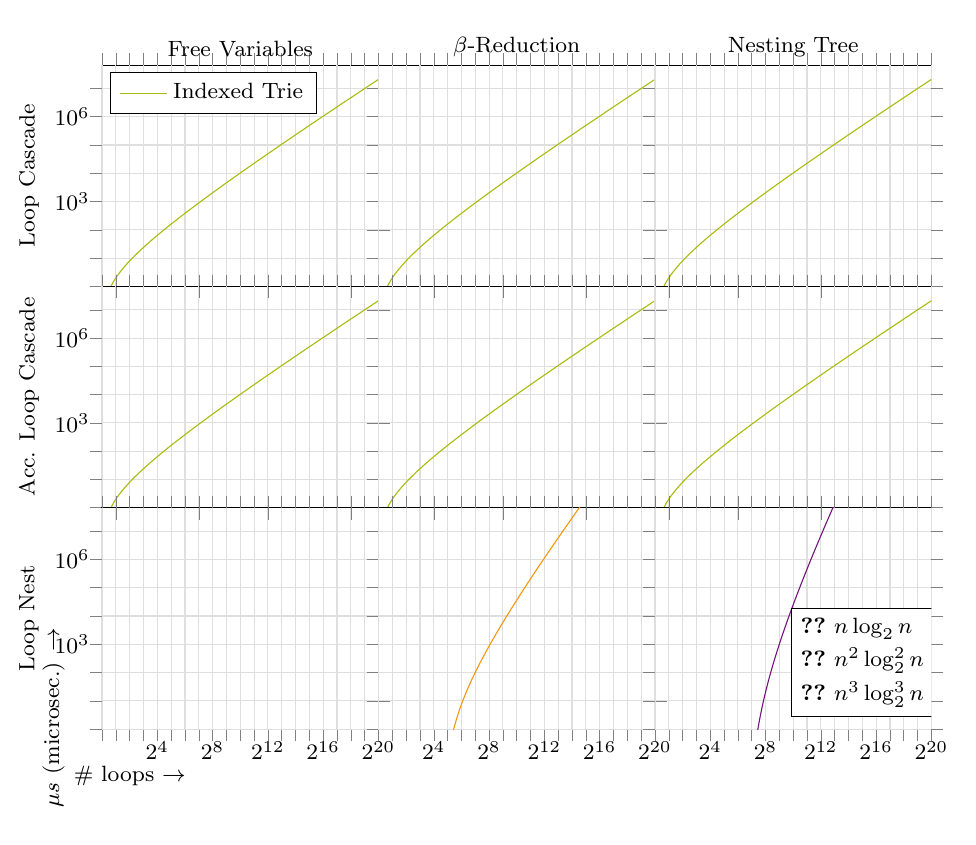
\begin{tikzpicture}
		\begin{groupplot}[
				group style={
						group size=3 by 3,
						horizontal sep=0cm,
						vertical sep=0cm,
						xlabels at=edge bottom,
						ylabels at=edge left,
						xticklabels at=edge bottom,
						yticklabels at=edge left,
					},
                title style={font=\footnotesize},
                tick align=outside,
                tick label style={font=\footnotesize, inner sep=0pt},
				width=.42\textwidth,   % each plot = 1/3 of textwidth
				% height=0.8*\dimexpr(\textwidth/3)\relax, % keep a reasonable aspect ratio
				% width=0.32\textwidth,
				% height=0.28\textwidth,
				log basis x={2},
				log basis y={10},
				grid=both,
				title style={yshift=-1.5ex},
                samples=100,
                domain=1:1048576,
				% ---- X AXIS ----
                xmode=log,
				% xlabel={Input Size $n$},
				xmin=1, xmax=1048576, % 2^0 .. 2^20
				xtickten={4,8,...,20}, % labels every 2 powers of 2
				xticklabel={\(2^{\pgfmathprintnumber{\tick}}\)},
				extra x ticks={1,2,4,8,16,32,64,128,256,512,1024,2048,4096,8192,16384,32768,65536,131072,262144,524288,1048576}, % all powers of 2
				extra x tick style={grid style={gray!25}, % faint grid
						tick label style={opacity=0}, % hide minor tick labels
					},
				% ---- Y AXIS ----
                ymode=log,
                ylabel style={font=\footnotesize, inner sep=-15pt},
				% ylabel={microseconds},
				ymin=1, ymax=67108864, % 2^0 .. 2^24
				ytickten={3,6,...,12}, % labels every 2 powers of 2
				yticklabel={\(10^{\pgfmathprintnumber{\tick}}\)},
				extra y ticks/.expanded={
                        1, 10, 100, 1000, 10000, 100000, 1000000,
                        10000000, 100000000
						% % generate all powers of 2 between 2^0 and roughly 2^40 (pgfplots ignores out-of-range)
						% 1,2,4,8,16,32,64,128,256,512,
						% 1024,2048,4096,8192,16384,32768,65536,131072,
						% 262144,524288,1048576,2097152,4194304,8388608,
						% 16777216,33554432,67108864,134217728,268435456,
						% 536870912,1073741824,2147483648,4294967296,
						% 8589934592,17179869184,34359738368,68719476736
					},
				extra y tick style={
						grid style={gray!25},
						tick label style={opacity=0},
					},
                legend pos=north west,
                legend style={font=\footnotesize},
			]

			% ---- Row 1: loop cascade ----
			\nextgroupplot[title={Free Variables}, ylabel={Loop Cascade}]

			\myplot{ACMPurple}{mark=*}{../trie.fvs.0.merged};
            \addlegendentry{Indexed Trie}

			\myplot{ACMBlue}{mark=*}{../set.fvs.0.merged};
            \addlegendentry{\texttt{std::set}}

			\myplot{ACMRed}{densely dashed, mark=triangle*}{../immer.fvs.0.merged};
            \addlegendentry{\immer}

            \addplot [ACMGreen, smooth] {x * ln(x) / ln(2)};
            % \addlegendentry{$n \log_2 n$}
            \label{nlogn}

			\nextgroupplot[title={$\beta$-Reduction}]

			\myplot{ACMPurple}{mark=*}{../trie.beta.0.merged};
			\myplot{ACMBlue}{mark=*}{../set.beta.0.merged};
			\myplot{ACMRed}{densely dashed,mark=triangle*}{../immer.beta.0.merged};

            \addplot [ACMGreen, smooth] {x * ln(x) / ln(2)};

			\nextgroupplot[title={Nesting Tree}]

			\myplot{ACMPurple}{mark=*}{../trie.nest.0.merged};
			\myplot{ACMBlue}{mark=*}{../set.nest.0.merged};
			\myplot{ACMRed}{densely dashed, mark=triangle*}{../immer.nest.0.merged};

            \addplot [ACMGreen, smooth] {x * ln(x) / ln(2)};

			% ---- Row 2: loop cascade2 ----
			\nextgroupplot[ylabel={Acc. Loop Cascade}]

			\myplot{ACMPurple}{mark=*}{../trie.fvs.1.merged};
			\myplot{ACMBlue}{mark=*}{../set.fvs.1.merged};
			\myplot{ACMRed}{densely dashed, mark=triangle*}{../immer.fvs.1.merged};

            \addplot [ACMGreen, smooth] {x * ln(x) / ln(2)};

			\nextgroupplot

			\myplot{ACMPurple}{mark=*}{../trie.beta.1.merged};
			\myplot{ACMBlue}{mark=*}{../set.beta.1.merged};
			\myplot{ACMRed}{densely dashed, mark=triangle*}{../immer.beta.1.merged};

            \addplot [ACMGreen, smooth] {x * ln(x) / ln(2)};

			\nextgroupplot

			\myplot{ACMPurple}{mark=*}{../trie.nest.1.merged};
			\myplot{ACMBlue}{mark=*}{../set.nest.1.merged};
			\myplot{ACMRed}{densely dashed, mark=triangle*}{../immer.nest.1.merged};

            \addplot [ACMGreen, smooth] {x * ln(x) / ln(2)};

			% ---- Row 3: loop nest ----
			\nextgroupplot[ylabel={Loop Nest}]

			\myplot{ACMPurple}{mark=*}{../trie.fvs.2.merged};
			\myplot{ACMBlue}{mark=*}{../set.fvs.2.merged};
			\myplot{ACMRed}{densely dashed, mark=triangle*}{../immer.fvs.2.merged};

            %\addplot [ACMPurple, smooth,domain=1:1024,xshift=24] {(((x * ln(x) / ln(2))^3};

			\nextgroupplot

			\myplot{ACMPurple}{mark=*}{../trie.beta.2.merged};
			\myplot{ACMBlue}{mark=*}{../set.beta.2.merged};
			\myplot{ACMRed}{densely dashed, mark=triangle*}{../immer.beta.2.merged};

            \plot [ACMOrange, smooth,domain=1:1024,xshift=24] {(x * ln(x) / ln(2))^2};
            \label{nlogn2}

			\nextgroupplot

			\myplot{ACMPurple}{mark=*}{../immer.nest.2.merged};
			\myplot{ACMBlue}{mark=*}{../set.nest.2.merged};
			\myplot{ACMRed}{densely dashed, mark=triangle*}{../immer.nest.2.merged};

            \plot [ACMPurple, smooth,domain=1:1024,xshift=34] {(x * ln(x) / ln(2))^3};
            \label{nlogn3}

            \node [draw,fill=white] at (rel axis cs: 0.75,0.3) {\shortstack[l]{
            \footnotesize\ref{nlogn} $n \log_2 n$ \\
            \footnotesize\ref{nlogn2} $n^2 \log_2^2 n$ \\
            \footnotesize\ref{nlogn3} $n^3 \log_2^3 n$}};

		\end{groupplot}
        \node[anchor=north east, rotate=90, align=center]
        at ($(group c1r3.south west) + (-2.5em,4em)$) {\footnotesize $\mu{}s$ (microsec.) $\to$};
        \node[anchor=north, align=center]
        at ($(group c1r3.south west) + (1em,-1em)$) {\footnotesize \# loops $\to$};
	\end{tikzpicture}
    % \vspace{-2ex}
	\caption{%
        Performance in $\mu{}s$ (microseconds) of free variables computation, $\beta$-reduction, and nesting tree computation, dependent on three synthetic programs with an increasing number of loops using the indexed trie and \immer (lower is better).
        $10^3\,\mu{}s$ correspond to $1\,\mathit{ms}$ (millisecond) and $10^6\,\mu{}s$ to $1\,s$ (second).%
    }
    \label{fig:bench}
\end{figure}

\end{document}
